% !TEX root = ../../prj4projektdokumentation.tex

\section{Kontrolmodul}
Kontrolmodulet består primært af to processer; En kommunikationsdel der kan håndtere at modtage data gennem en TCP forbindelse og konvertere disse data til noget der kan bruges i resten af programmet, herunder også HMI delen. En styringsdel der kan bruge disse data i styringen af trinskifteren.

Kontrolmodulet er programmmeret på en Siemens S7-1200 PLC med en 1214C DC/DC/DC CPU og signalmodulet AQ1x12BIT. Sammen med PLC'en sidder en switch af typen CSM 1277 .


\subsection{TCP kommunikation}
\label{sec:TCPkommunikation}
Kontrolmodulet er lavet som en client i forhold til kommunikationsmodulet, der er server. Den sender altså en forespørgelse på at modtage data til kommunikationsmodulet, hvorefter den modtager ny data fra den forespurgte enhed. Mere om selve protokollen kan findes i afsnit \ref{sec:TCPprotokol} TCP protokol. Det er kontrolmodulet der oprette TCP forbindelse og står for at nedlægge den igen.

TCP komunikationen er opdelt i 4 FC'er; OpretForbindelse, SendData, ModtagData og AfslutForbindelse. Simatic TIA portal har nogle indbyggede open user comunication  blokke, der kan bruges til LAN kommunikation.

OpretForbindelse består af funktionsblokken TCON, som er vist på figur \ref{fig:TCON}. Når der på REQ ses en rising edge, vil den forsøge at oprette forbindelse til en bestemt IP adresse og opretholde den, også selvom REQ bliver sat 0 igen. Forbindelsen bliver vedligeholdt automatisk asynkront, så programmet kan udføre andet samtidigt. Hvis forbindelsen bliver brudt, skal REQ have en rising edge før TCON vil forsøge at oprette forbindelse igen. Datablokken Ethernet er oprettet med henblik på at indeholde globale statics anvendt i forbindelse med TCP kommunikationen, da FC'er ikke har nogen hukommelse fra scan til scan.

ID er identifikationen på forbindelsen internt i PLC'en, som de resterende blokke bruger til at identificere hvilken forbindelse de er tilknyttet, hvis der skulle være flere. Her er ID sat til 1, da der kun er en forbindelse til kommunikationsmodulet.

CONNECT parameteren er en pointer til data området der indeholder forbindelsesinformation. TCON muliggør at få informationer om forbindelsen tilstand gennem DONE, BUSY, ERROR og STATUS. Disse outputs ligger i den tilhørende DB TCON\_DB og kan kaldes gennem den. I dette projekt er der dog ikke udviklet nogen form for fejlhåndtering og disse outputs anvendes ikke. Der henvises til bilag B-2,kapitel 11, for mere dybdegående forklaring af disse.

\begin{figure}[H] % (alternativt [H])
	\centering
	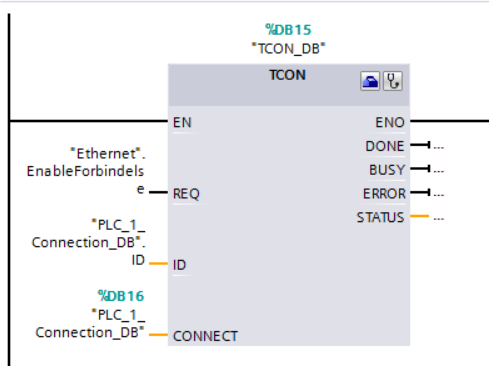
\includegraphics[width=0.5\textwidth]{Figure/TCON}
	\caption{TCON brugt i funktionen OpretForbindelse}
	\label{fig:TCON}
\end{figure}

Selve konfigureringen af hvilke enheder(IP adresser) kommunikationen skal foregå imellem sættes under properties for TCON. På figur \ref{fig:Konfiguration} kan det kan ses at på lokalsiden er PLC'en sat op til at have IP adressen 192.168.0.120, anvende TCP over subnet PN/IE\_1, som er default 255.255.255.0, samt være aktiv i forhold til at oprette forbindelsen. Feltet Connection data, fortæller hvilken Datablok der indeholder data omkring forbindelse, herunder bla. ID og CONNECT.

På partnersiden er Arduinoen ikke et Siemens modul og derfor unspecified. Her er valgt at kommunikationsmodulet har IP adressen 192.168.0.129 og bruger port 27015 til kommunikationen. Denne port er valgt af hensyn til Arduinoens præferencer i forhold til mulige porte.

\begin{figure}[H] % (alternativt [H])
	\centering
	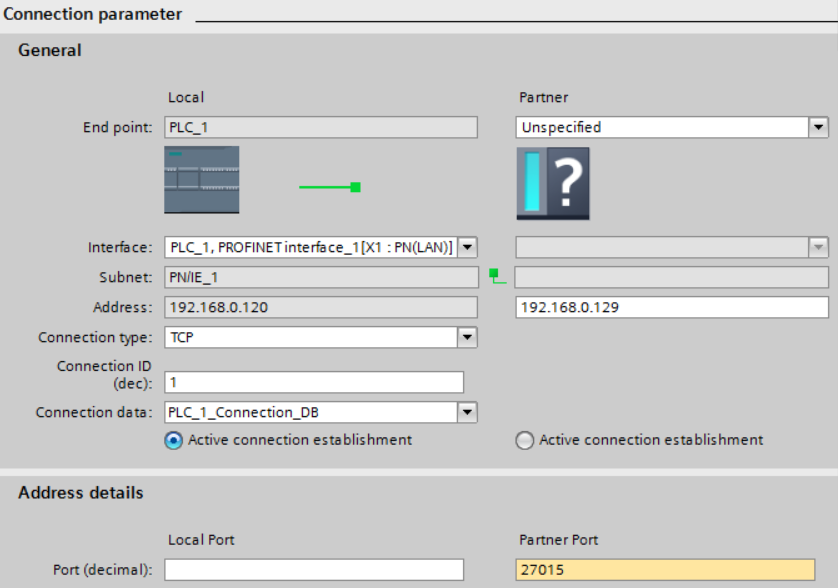
\includegraphics[width=0.7\textwidth]{Figure/KonfigurationAfTCPforbindelse}
	\caption{Konfiguration af TCP forbindelse}
	\label{fig:Konfiguration}
\end{figure}

Funktionen AfslutForbindelse står for at nedlægge forbindelse. Da der kun kommunikeres med en enhed, anvender programmet aldrig denne mulighed. Alligevel er funktionen lavet for at det er nemt at videreudvikle, med henblik på at tilføje flere TCP forbindelser. 

Funktionsblokken TDISCON anvendes til denne opgave. Når blokkens REQ ser en rising edge nedlægges forbindelsen og det vil kræve en rising edge på TCON's REQ for at genetablere forbindelsen. Blokken skal også bruge et ID på forbindelsen, ID'et er sat i konfigurationen af TCON. Igen kan informationer omkring blokken fåes gennem DONE, BUSY, ERROR og STATUS. Disse anvendes ikke, da der ikke er lagt vægt på fejlhåndtering i dette projekt. De kan kaldes gennem datablokken TDISCON\_DB. Der henvises til bilag B-2, kapitel 11 for mere dybdegående forklaring af disse.

\begin{figure}[H] % (alternativt [H])
	\centering
	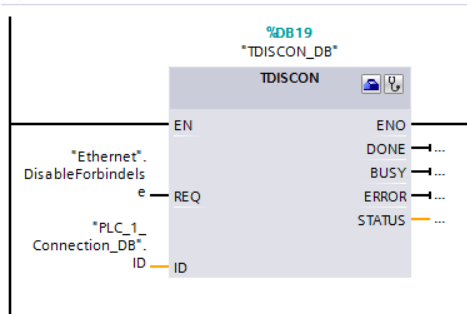
\includegraphics[width=0.5\textwidth]{Figure/TDISCON}
	\caption{TDISCON brugt i funktionen AfslutForbindelse}
	\label{fig:TDISCON}
\end{figure}

Når forbindelsen er oprettet bruges funktionerne SendData og ModtagData til  kommunikering af data. SendData anvender funktionsblokken TSEND til at afsende data placeret i den globale static SendData. Når REQ modtager en rising edge afsendes dataet. Mens ID specificerer hvilken forbindelse, der skal sendes over.

Ligesom TCON og TDISCON anvendes DONE, BUSY, ERROR og STATUS ikke. Der henvises til bilag B-2, kapitel 11 for mere dybdegående forklaring af disse.

\begin{figure}[H] % (alternativt [H])
	\centering
	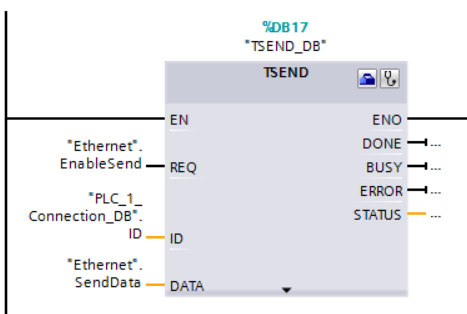
\includegraphics[width=0.5\textwidth]{Figure/TSEND}
	\caption{TSEND brugt i funktionen SendData}
	\label{fig:TSEND}
\end{figure}

Til at styre hvor ofte der forespørges ny data og hvilken enhed der forespørges data fra, er designet et netværk, hvor en global static boolean Firsttime sættes true før send processen går igang. Firsttime bliver sat true når data er modtaget og gemt. Den er defualt true ellers vil det blokere programmet i kraft af at PLC'en ikke modtager data før den har sendt en kommando på ny data.

Når Firsttime er true igangsættes netværket vist på figur \ref{fig:ValgAfEnhedSend}. Her resettes den static der styrer REQ på TSEND og en on delay timer, SendDataTimer, startes. Timere anvendes i programmet for kunne styre hvor ofte der hentes ny data. For systemet der udvikles er det ikke nødvendigt at dette går hurtigt. Så det blev besluttet at data fra både den centrale og den decentrale måleenhed skulle opdateres hver 2 sekunder. Derfor er der valgt en timer på 500ms i både SendData og ModtagData funktionen. Hvilket resultere i 1 sekund pr enhed og 2 sekunder samlet.

Når SendDataTimers udgang går true, resettes Firsttimer til false og den gloable static EnhedToReq sammenlignes med to konstanter 15 og 240, som svarer til Måleenhed Central og Måleenhed Decentral. Disse værdier er valgt da de er 1's komplement af hinanden. Så når de forespurgte data er modtagede og gemt kan man skifte EnhedToReq ved at invertere den unsigned integer.


Til sidst på figur \ref{fig:ValgAfEnhedSend} flyttes kommandoen for den valgte enhed over i SendData, som er det char array der sidder på TSEND's DATA ben og REQ sættes true via EnableSend boolean.

\begin{figure}[H] % (alternativt [H])
	\centering
	\includegraphics[width=1\textwidth]{Figure/valgAfEnhedSend}
	\caption{Netværket der styrer hvilken enhed der forespørges data fra}
	\label{fig:ValgAfEnhedSend}
\end{figure}

ModtagData funktionen er opbygget på meget samme måde som SendData funktionen med en funktionsblok TRCV vist på figur \ref{fig:TRCV} til selve TCP kommunikation og et netværk deisgnet til at gemme det modtagede data. Netværket kan ses på figur \ref{fig:GemModtagetdata}. TRCV er opbygget med en EN\_R, der så længe den er true vil modtage data. Den globale static EnableModtag er default true, da funktionsblokken bliver udført asynkront, så den vil ikke blokkere programmet herved. Ligeså snart en forespørgelse på ny data er sendt er programmet altså klar til at modtage et svar.

ID er det samme som for de resterende kommunikationsblokke. DATA dækker over hvor modtaget data skal gemmes. Som i de resterende blokke anvendes outputs ikke. Der henvises til bilag B-2, kapitel 11 for mere dybdegående forklaring af disse.

\begin{figure}[H] % (alternativt [H])
	\centering
	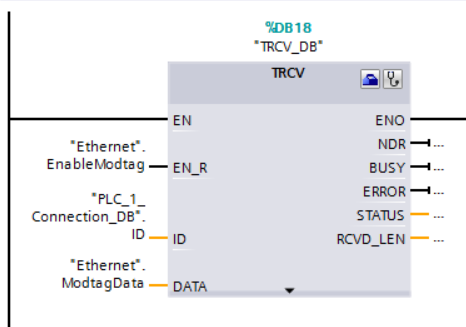
\includegraphics[width=0.5\textwidth]{Figure/TRCV}
	\caption{TRCV brugt i funktionen ModtagData}
	\label{fig:TRCV}
\end{figure}

Ligeså snart SendDataTimers output går true, sættes Firsttime false, hvilket sætter gem modtagede data netværket igang. Her er placeret ModtagDataTimer, som også er en on delay timer. Når dens output går true, vælges i hvilket global static word array, DataCentralEnhed og DataDecentralEnhed, dataet skal gemmes. Disse anvendes i forbindelse med HMI'et. Se afsnit \ref{sec:HMI}. Hvilket der bliver valgt afhænger igen af EnhedToReq. Samtidig sættes Firsttimer true, så data igen kan forespørges i SendData funktionen. Den global static boolean Invert, anvendes til den tidligere beskrevne invertering af EnhedToReq. Dette sker i et seperat netværk til sidst i ModtagData funktionen, hvor en true Invert muliggør invertering ved hjælp af en funktion INV og sætter Invert false.

SendData og ModtagData funktionerne looper altså i en evig løkke, hvor Måleenheden der forespørges data fra efter hver runde skiftes.

\begin{figure}[H] % (alternativt [H])
	\centering
	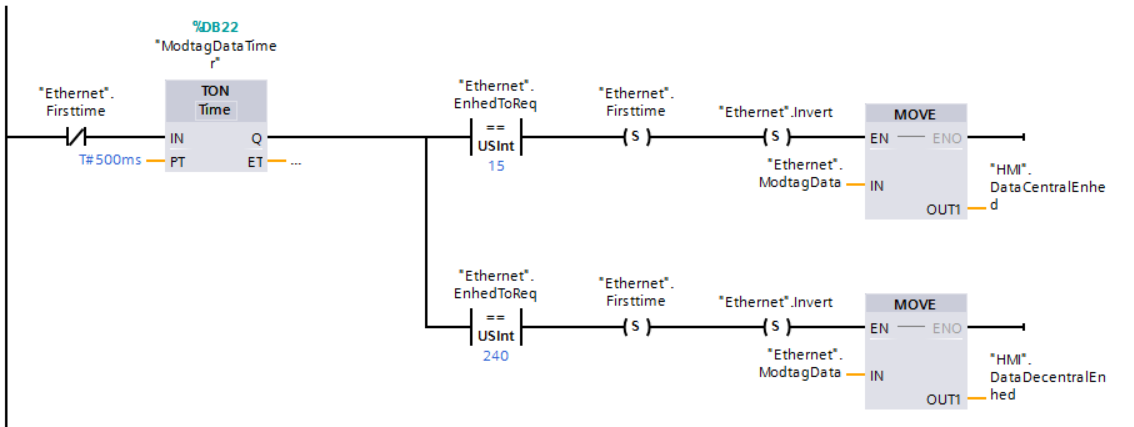
\includegraphics[width=1\textwidth]{Figure/GemModtagetData}
	\caption{Netværket der gemmer modtagede data}
	\label{fig:GemModtagetdata}
\end{figure}

I dette program er der kun en OB, OB1, der eksekveres, de fire funktioner OpretForbindelse, SendData, ModtagData og AfslutForbindelse ligger herfor i OB1 i det ene netværk af to. Det andet netværk indeholder styringen af trinskifteren og indeholder en FB; trinskifter.

\subsection{Styring af trinskifteren}

FB'en trinskifter har et input og tre outputs. Input i form af DataDecentralEnhed[1]. På plads et i word arrayet ligger information omkring spændingen målt ude ved den decentrale Målenhed også benævnt Forbruger 1. Output er tre booleans Trin 1, Trin 2 og Trin 3, der hver er forbundet med et output på PLC'en, henholdsvis Q0.6, Q0.7 og Q1.0. Se figur \ref{fig:PLCTrinskifter}.

\begin{figure}[H] % (alternativt [H])
	\centering
	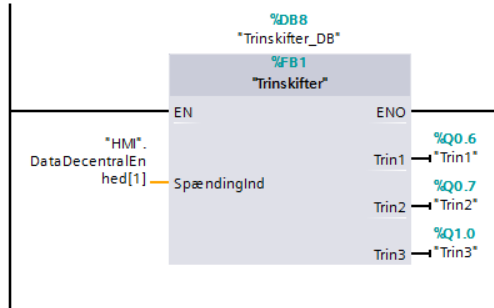
\includegraphics[width=0.5\textwidth]{Figure/PLCTrinskifter}
	\caption{FB'en Trinskifter}
	\label{fig:PLCTrinskifter}
\end{figure}

Trinskifter består af 13 netværk, 1 initieringsnetværk, 5 automatisk mode netværk og 7 manuel mode netværk. Disse eksekveres i sekvenser, styret af den lokale static integer Step. Netværk 1 er et initieringsnetværk, der sætter Trin2 true og sætter Step til 2 med funktionen MOVE. Step 2 svarer til at systemet er i Trin 2 i automatisk tilstand. Trin 2 i koden er Trin 5 på trintransformeren.

På figur \ref{fig:Trin2AutomatiskMode} ses det netværk i den automatiske del, hvor udgangen Trin 2 er sat. Trin er her en static, der bruges i HMI'et. Se afsnit \ref{sec:HMI}. For at undgå at programmet kan nå at lave et multistep, altså f.eks. fra Trin 1 til Trin 3, er sat en on delay timer, Trin2VentTilNyData. Konstanten VentTid er sat til 2,5 sekunder, hvilket er mere end de 2 sekunder der går før der er ny data. Dermed får man ny data fra et nyt stabilt niveau efter et trinskift og programmet vil altså ikke skifte endnu et trin grundet gamle målingerne.

Programmet står og venter efter timeren. Her kan man ved hjælp en trykknap på HMI'et skifte til ManuelMode. Ved et tryk bliver ManuelMode true og Step bliver sat til 12, som svarer til Trin 2 i manuel mode. Se figur \ref{fig:Trin2ManuelMode}. Hvis en bruger ikke interagerer med systemet, vil inputtet, den unsigned integer SpændingInd, blive sammenlignet med to konstanter 4400 og 3600. Disse to værdier svarer til 10\% over og under det ønskede spændingsniveau på 4000mV. Hvis målinger fra Måleenhederne skulle komme udenfor dette interval vil der bliver skiftet trin. Afhængig af om det er et trin ned eller op MOVES henholdsvis 3 eller 4 over i Step.
Et trinskift op er vist på figur \ref{fig:Trin2SkiftOp}.

\begin{figure}[H] % (alternativt [H])
	\centering
	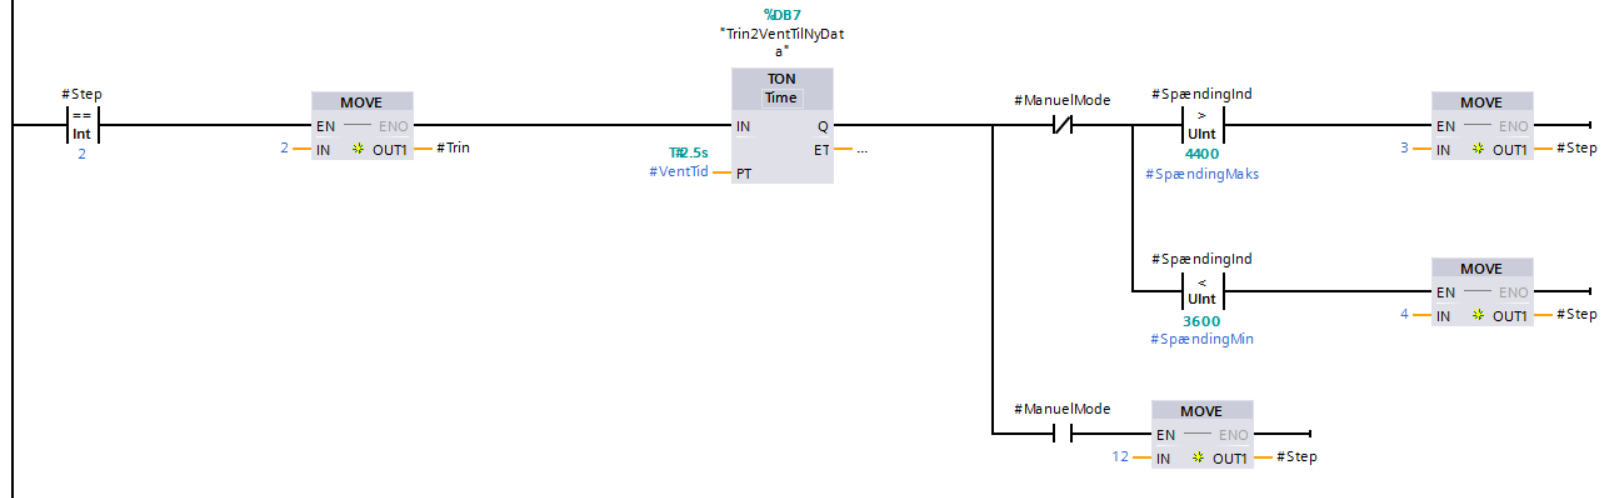
\includegraphics[width=1\textwidth]{Figure/Trin2AutomatiskMode}
	\caption{Trin 2 i automatisk mode}
	\label{fig:Trin2AutomatiskMode}
\end{figure}

I manuel mode er konceptet ikke at trinskiftene skal styres af spænidngsmålinger, men af brugeren gennem HMI'et. Der er derfor i stedet for sammenligningerne af SpænidngInd placeret to booleans KnapOp og KnapNed. Hvis en af disse bliver true vil programmet skifte trin enten op eller ned. De manuelle skift ligger i Step 13 og 14 for trin 2. I manuel mode trin 2 er det også muligt for brugeren igen at aktivere Automatisk mode og springe tilbage til Step 2.

\begin{figure}[H] % (alternativt [H])
	\centering
	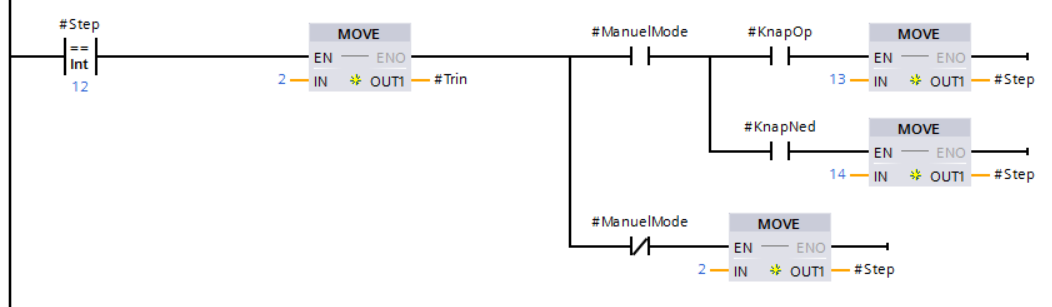
\includegraphics[width=1\textwidth]{Figure/Trin2ManuelMode}
	\caption{Trin 2 i manuel mode}
	\label{fig:Trin2ManuelMode}
\end{figure}

Hvordan et trinskift udføres i programmet er gennemgående det samme, forskellen ligger i hvilke trin der skiftes imellem og om det er et skift op eller ned. Dette gælder både for manuel og automatisk mode.

Herunder er derfor kun vist et eksempel på et trinskiftnetværk. De resterende og resten af programmet kan findes i bilag A-2. Dette eksempel er et trinskift op fra trin 2 til trin 3. For at sikre at der altid er forsyning på distributionslinjen skal der altid være et trin på transformeren der er aktivt. Derfor er en on delay timer, TrinSkift2til3, anvendt. Det nye trin, i dette tilfælde trin 3 sættes true, så snart Step bliver 4, mens det gamle trin resettes efter 2 sekunder, hvorefter Step bliver sat til 5 og systemet er nu sikkert og uden afbrydelser blevet flyttet til et nyt trin. For flere kredsløbsdetaljer om skiftet på selve transformeren, henvises til afsnit \ref{sec:Trinskifter}.

\begin{figure}[H] % (alternativt [H])
	\centering
	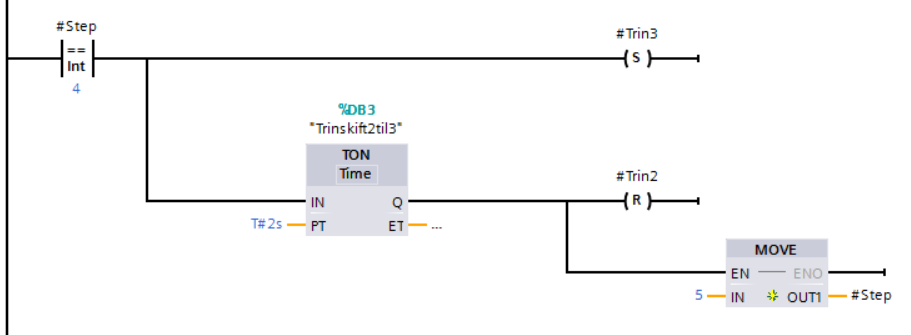
\includegraphics[width=0.8\textwidth]{Figure/Trin2SkiftOp}
	\caption{Trin 2 skift et trin op}
	\label{fig:Trin2SkiftOp}
\end{figure}

Det er værd at bemærke at det kun er i trin 2 at systemet kan skifte både op og ned, fordi der kun er 3 trin i systemet. Der kan derfor kun skiftes op fra trin 1 og kun skiftes ned fra trin 3. Grunden til at der er 5 netværk i automatisk mode og 7 i manuel mode, er at trin 1's og trin 3's trinskift ligger i selve trinets netværk. Koden er meget lig det forklarede trinskift, men placeret lige efter sammenligningen af SpændingInd.